%% LaTeX-Beamer template for KIT design
%% by Erik Burger, Christian Hammer
%% title picture by Klaus Krogmann
%%
%% version 2.1
%%
%% mostly compatible to KIT corporate design v2.0
%% http://intranet.kit.edu/gestaltungsrichtlinien.php
%%
%% Problems, bugs and comments to
%% burger@kit.edu

\documentclass[18pt, xcolor=table]{beamer}

%% SLIDE FORMAT

% use 'beamerthemekit' for standard 4:3 ratio
% for widescreen slides (16:9), use 'beamerthemekitwide'
\usepackage[utf8]{inputenc}
\usepackage[T1]{fontenc}
\usepackage{templates/beamerthemekit}
\usepackage{tabularx}
%\usepackage{templates/beamerthemekitwide}

%% TITLE PICTURE

% if a custom picture is to be used on the title page, copy it into the 'logos'
% directory, in the line below, replace 'mypicture' with the 
% filename (without extension) and uncomment the following line
% (picture proportions: 63 : 20 for standard, 169 : 40 for wide
% *.eps format if you use latex+dvips+ps2pdf, 
% *.jpg/*.png/*.pdf if you use pdflatex)

\titleimage{controller}

%% TITLE LOGO

% for a custom logo on the front page, copy your file into the 'logos'
% directory, insert the filename in the line below and uncomment it

\titlelogo{ElipseLogo}

% (*.eps format if you use latex+dvips+ps2pdf,
% *.jpg/*.png/*.pdf if you use pdflatex)

%% TikZ INTEGRATION

% use these packages for PCM symbols and UML classes
\usepackage{templates/tikzkit}
% \usepackage{templates/tikzuml}

% the presentation starts here

\title[Elipse]{Elipse -- Einteilungs Interface für das PSE}
\subtitle{Implementierungspräsentation}
\author{D. Biester, E. Dohse, P. Faller, P. Loth, L. Seufert, S. Kopmann}

\institute{IPD Snelting}

% Bibliography

\usepackage[citestyle=authoryear,bibstyle=numeric,hyperref,backend=biber]{biblatex}
\addbibresource{templates/example.bib}
\bibhang1em
\beamertemplatenavigationsymbolsempty

\begin{document}

% change the following line to "ngerman" for German style date and logos
\selectlanguage{ngerman}

%title page
\begin{frame}
\titlepage
\end{frame}
\section{Überblick}
\begin{frame}{Überblick}
\begin{itemize}
  \item Auszüge aus den implementierten Funktionen
  \item Zeitplan
  \item Probleme bei der Implementierung
  \item Änderungen gegenüber dem Entwurf
  \item Statistiken
\end{itemize}
\end{frame}

\section{Implementierte Funktionen}
\begin{frame}{Auszüge aus den Implementierten Funktionen}
\begin{itemize}
  \item E-Mail-Benachrichtigung mit Konfiguration über die Webseite
  \item Einteilungs-Warteschlange
  \item Güte- und Einteilungskriterien könne über den Java ServiceLoader geladen werden
  \item Undo-Funktion beim Einteilungsergebnisändern
  \item Registrierte Studenten aus vorherigen Semester können Account behalten und müssen nur ihre Studiendaten aktualisieren.
  \item Verifizieren der E-Mail-Adresse und Passwort Zurücksetzen-Funktion
\end{itemize}
\end{frame}

%Sehr wilde Hacks um Layout anzupassen

\section{Zeitplan}
\begin{frame}[plain]{Zeitplan}
\begin{table}[H]
\begin{tabularx}{\textwidth}{l|l X X X}
\hline
 	& 1. Woche			& 2. Woche		& 3. Woche & 4. Woche\\
\hline 
Daniel	& Views			& Views \phantom{+} Controller  pac4j & Layout \phantom{++} Verificator & Tests \phantom{++} Bugfixes \\
\hline
Sam & Views&Views \phantom{+} Controller & QualityCriteria  Notification & Tests \phantom{++} Bugfixes \\
\hline
Philipp Faller&Data&Import/Export
Index\-Controller&Admin\-Controller&Tests \phantom{++}
Bugfixes \\
\hline
Philipp Loth&Allocator&Import/Export
Index\-Controller&Admin\-Controller&Tests \phantom{++}
Bugfixes \\
\hline
Emil&Allocator&Allocator&Admin\-Controller&Tests \phantom{++}
Bugfixes \\
\hline
Lars&Data&Data \phantom{++} (Ebean)&Adviser\-Controller&Tests \phantom{++}
Bugfixes 
\end{tabularx}
\end{table}
\end{frame}

\newcommand{\mehr}{\cellcolor{white!90!green}}
\newcommand{\weniger}{\cellcolor{white!90!red}}

\subsection{Änderungen}
\begin{frame}[plain]{Änderungen}
\begin{table}[H]
\begin{tabularx}{\textwidth}{l|l X X X}
\hline
 	& 1. Woche			& 2. Woche		& 3. Woche & 4. Woche\\
\hline 
Daniel	& Views			& \weniger Views \phantom{+} Controller & \mehr Layout \phantom{+} Verificator
\phantom{+} pac4j&\weniger Deadlines Bugfixes \\
\hline
Sam & Views&\weniger Views& QualityCriteria Notification & Tests \phantom{++} Bugfixes \\
\hline
Philipp Faller&Data&\weniger Data&\weniger Bugfixes&\weniger Bugfixes\\
\hline
Philipp Loth&Allocator&\weniger Import/Export
&\weniger Import/Export &\weniger \weniger Tests \phantom{++} Bugfixes Form-Validation\\
\hline
Emil&Allocator&\mehr Controller&\mehr Controller&\weniger Form-Validation Bugfixes\\
\hline
Lars&Data&Data \phantom{++} (Ebean)&\weniger Controller \phantom{+} Daten &
\weniger Controller \phantom{+} Bugfixes \\
\end{tabularx}
\end{table}
\end{frame}

\section{Probleme bei der Implementierung}
\begin{frame}{Probleme bei der Implementierung}
\begin{itemize}
  \item Fehlende oder falsche Dokumentation der verwendeten Bibliotheken und Frameworks
  \item unerwartete Fehler durch E-Bean
  \item Pac4J Implementierung
\end{itemize}
\end{frame}

\section{Änderungen zum Entwurf}
\begin{frame}{Änderungen zum Entwurf}
\begin{itemize}
  \item Hinzugefügte Klassen und Pakete
  \begin{itemize}
    \item Security-Packet (Authentifizierung und Passwort-Encryption)
    \item Formular-Validierung
    \item Passwort-Resetter und E-Mail-Verifizierer
  \end{itemize}
\end{itemize}
\end{frame}

\begin{frame}{Statistik}
\vspace*{-7mm}
\begin{figure}
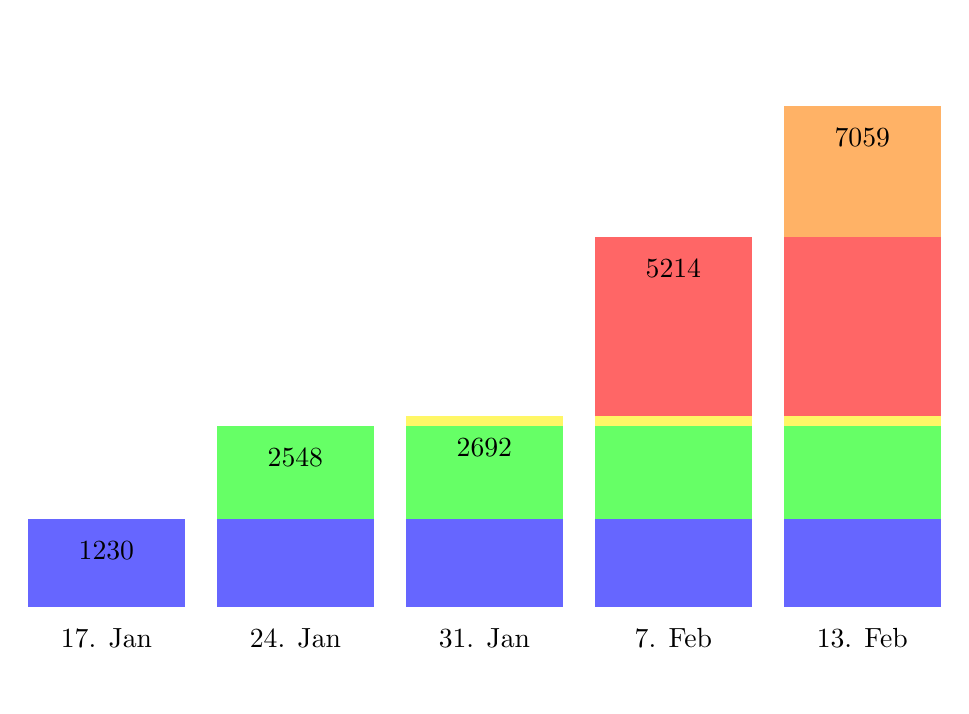
\begin{tikzpicture}[x={(0.8mm,0mm)},y={(0mm,0.9mm)}]
\draw[yshift=-4mm] (0,0) node{17. Jan} (30, 0) node{24. Jan} (60, 0) node{31. Jan} (90, 0) node{7. Feb} (120, 0) node{13. Feb};
\draw[line width=20mm,orange!60] (0,0) plot [ycomb]
coordinates {(120,70.59)};
\draw[line width=20mm,red!60] (0,0) plot [ycomb]
coordinates {(120,52.14) (90,52.14)};
\draw[line width=20mm,yellow!60] (0,0) plot [ycomb]
coordinates {(120,26.92) (90,26.92) (60,26.92)};
\draw[line width=20mm,green!60] (0,0) plot [ycomb]
coordinates {(120,25.48) (90,25.48) (60,25.48) (30,25.48)};
\draw[line width=20mm,blue!60] (0,0) plot [ycomb]
coordinates {(120,12.30) (90,12.30) (60,12.30) (30,12.30) (0,12.30)};
\draw[yshift=-4mm](0,12.30) node{1230} (30, 25.48) node{2548} (60, 26.92) node{2692} (90, 52.14) node{5214} (120, 70.59) node{7059};

\end{tikzpicture}
\end{figure}
\end{frame}

\appendix
\beginbackup

\begin{frame}{Fragen}
\printbibliography
\end{frame}

\backupend

\end{document}
